
\documentclass[submit, techrep]{ipsj}
%\documentclass{ipsj}

\usepackage[dvipdfmx]{graphicx}
\usepackage{latexsym}
\usepackage{color}
\usepackage{amsmath}
\usepackage{siunitx}
\usepackage{here}

\input{00_macro}

\def\Underline{\setbox0\hbox\bgroup\let\\\endUnderline}
\def\endUnderline{\vphantom{y}\egroup\smash{\underline{\box0}}\\}
\def\|{\verb |}


\setcounter{巻数}{59}
\setcounter{号数}{1}
\setcounter{page}{1}

%\makeatletter
%\pagestyle{empty}
%\def\@oddhead{}%
%\def\@evenhead{}%
%\def\ps@IPSJTITLEheadings{}
%\makeatother







\begin{document}


\title{GUI操作における膝入力の応用可能性の調査}



\affiliate{CS1}{筑波大学 \\システム情報工学研究科 コンピュータサイエンス専攻}
\affiliate{CS2}{筑波大学 システム情報系}


%\paffiliate{JU}{情報処理大学\\
%Johoshori University}

\author{市川 佑}{}{CS1}[yichikawa@iplab.cs.tsukuba.ac.jp]
\author{志築 文太郎}{}{CS2}[shizuki@cs.tsukuba.ac.jp]
\author{高橋 伸}{}{CS2}[shin@cs.tsukuba.ac.jp]

\begin{abstract}
これまで我々は距離センサアレイを用いた膝によるカーソル操作を実現し,その特性を調査してきた.
しかし,一般的なGUI操作に対する膝操作の適用については未検証であった.
本稿では,ペイントツールに膝操作を適用することで,一般的なGUIへの適用可能性を探った.
今回,膝による操作の例として,ベジェ曲線の制御点の移動,
レイヤの切り替え,ペンの色の切り替えを実装した.
また,実装したペイントツールを用いて複数レイヤの描画を行う実験を行い,
膝による操作のユーザビリティ評価を行った.
\end{abstract}






\maketitle

%1
\section{はじめに}
%一般に椅子に座り机上でコンピュータを用いて作業をする場合,両手をマウスやキーボードの操作に充てることが多い.
一般にGUIアプリケーションは,マウスやタッチによる入力により操作することが多い.
一方で,足は操作が割り当てられることは少なく,ほとんど動かすことがない.
操作を足に割り当てることができれば,
手が荷物で塞がっている状況\cite{Fan:2017:ESF:3123021.3123043}や,電車内など手の動きが制限されてしまう状況\cite{Fukahori:2015:ESF:2702123.2702308}でも端末の操作を行うことができ,さらに手と足を組み合わせた操作の拡張も可能となる.\par
%1960 年代から存在している\cite{1698228}が,現在は手による操作が中心である.
足による操作を用いたコンピュータ向けインタフェースの研究は昔から行われており,先行研究には膝でレバーを操作する方法\cite{1698228},机に取り付けた装置を足で動かす方法\cite{Pearson:1986:MMD:22627.22392, Pearson:1988:EEP:57167.57169}や,足の位置によって摩擦力を変えることができる機構を取り付けた靴\cite{Horodniczy:2017:FHE:3025453.3025625}を用いる方法がある.
こうした方法は,大型な装置を用いる,あるいは身体の一部に装置を取り付けるものであるため,設置に時間がかかる,ユーザの衣服などに制限が生じるといった制約がある.\par
またこれらの研究では,一般のGUIアプリケーションを使った足や膝のユーザビリティについての調査は行われていない.
我々の以前の研究\cite{weko_196526_1}では,距離センサアレイを机下に設置することで膝の位置を認識することでカーソル操作を行い(\refImg{system_image}),膝操作の特性を調査した.その結果,膝操作はタッチパッド,ジョイスティックに匹敵する性能があり,疲労感はあるが,無理なく意図した通りに行うことができると分かった.しかし,一般的なGUI操作に対して膝操作を適用した場合については未検証であった.\par
そこで,本稿では一般のGUI操作へ膝操作を適用し,膝操作が適合する操作,およびアプリケーション実装上での指針を明らかにすることを目的とする.このアプローチとして,ベジェ曲線描画プログラムをアプリケーション例として,各機能に膝操作を適用し,ユーザスタディを行う.
\begin{figure}[h]
	\begin{center}
		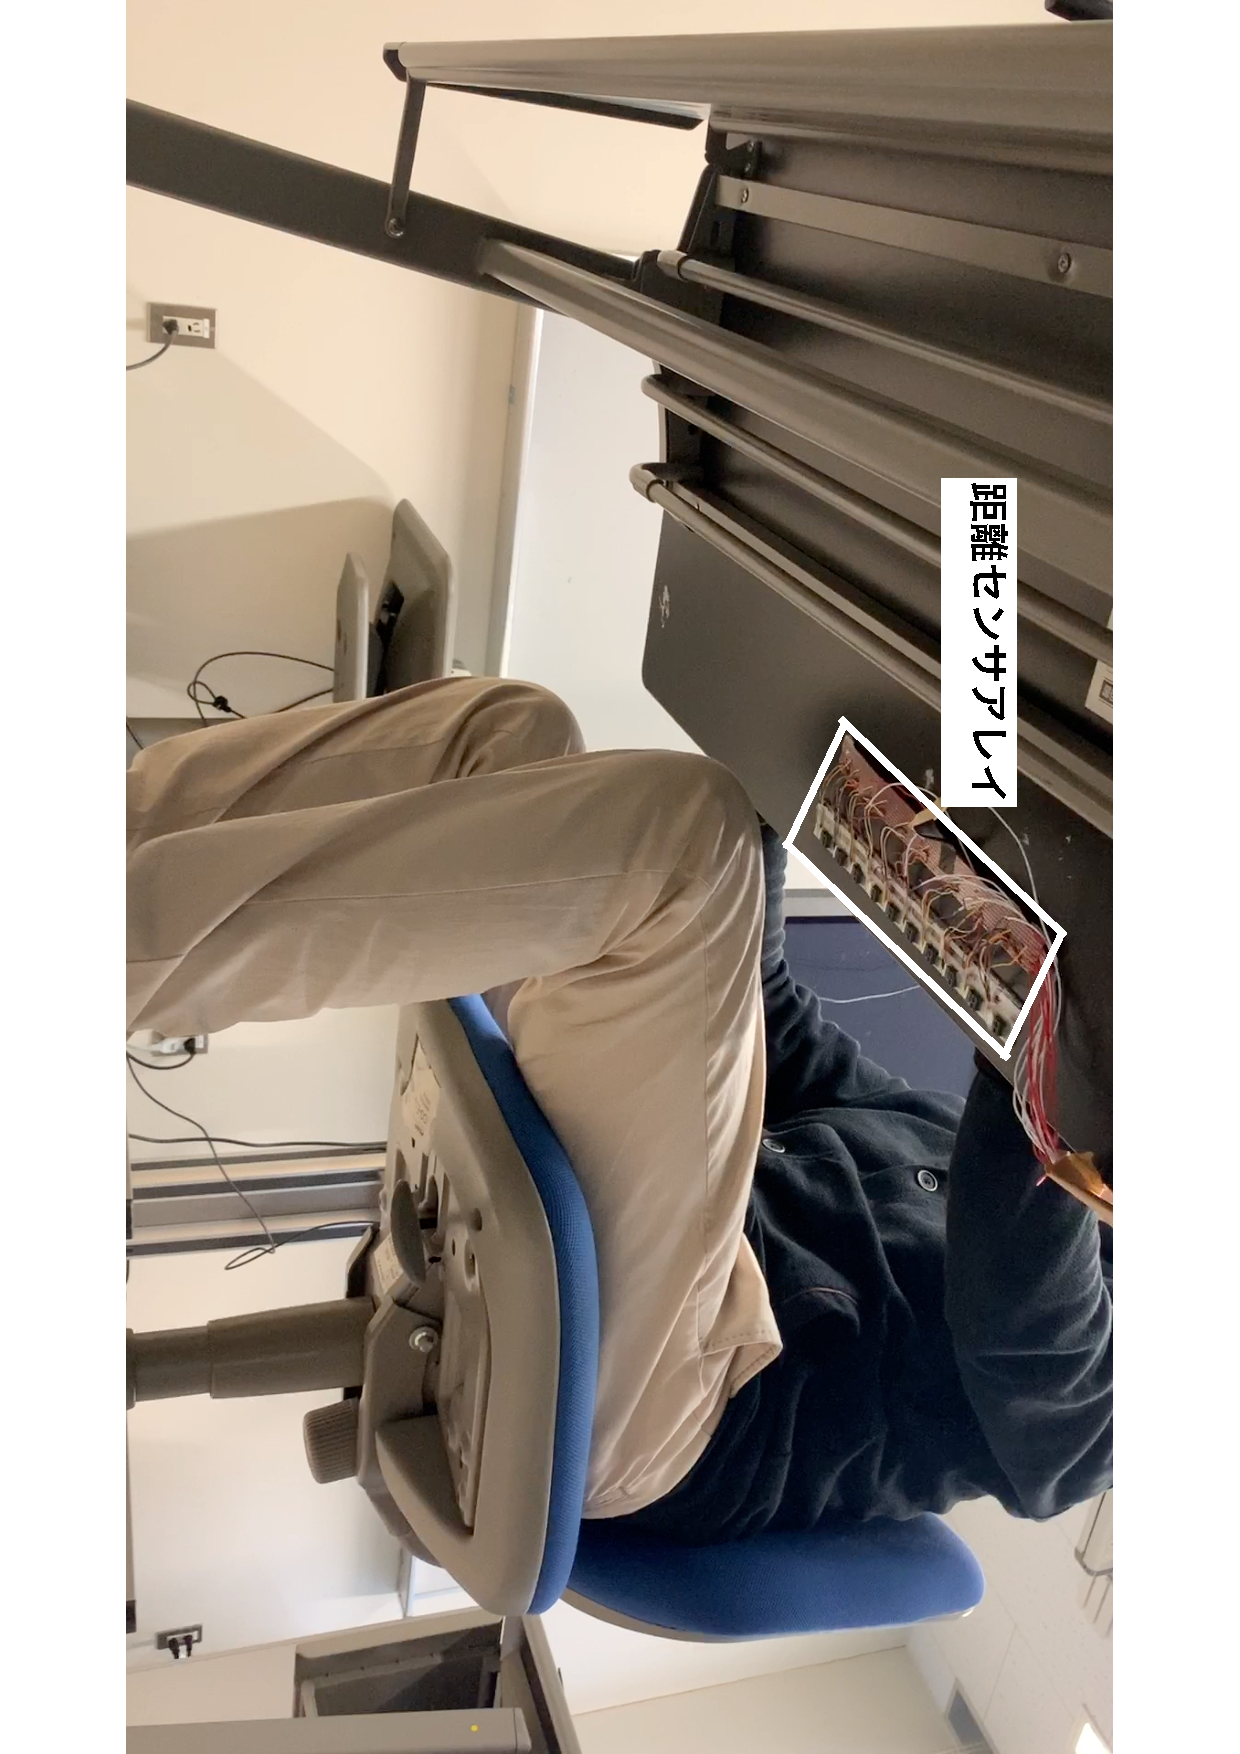
\includegraphics[width = 0.7\hsize, angle = 90]{./figures/system_image_2.pdf}
	\end{center}
	\caption{距離センサアレイと膝での操作の様子}
	\label{img:system_image}
\end{figure}


\section{関連研究}
関連する研究について,座った状態において足を入力として用いている研究と,膝を入力として用いた研究を挙げる.

%\subsection{足を用いたジェスチャ入力}
%Fanら\cite{Fan:2017:ESF:3123021.3123043}は,足のジェスチャによりモバイル端末を操作することに対する実証研究を行った.
%荷物を持ったまま,ユーザ定義の足のジェスチャを用いて操作する方法と,荷物を降ろして手で端末を持ち操作する方法を比較したところ,前者の方が70\%高速な操作が可能であるという結果となった.
%HanらのKick\cite{Han:2011:KIU:2037373.2037379}では,キックジェスチャを端末操作に用いるために,ユーザがキックの方向と速度をどの程度操作できるかを調査した.
%Fukahoriら\cite{Fukahori:2015:ESF:2702123.2702308}は複数の圧力センサを靴下に搭載することで,足の荷重を認識し,電車内といった公共スペースにおけるコンピュータの制御に用いた.\par
%\fixme{本研究は,屋内での利用のみを想定した環境設置型の装置を用いるという点で異なっており,屋内であっても足を用いたインタラクションは有効であると考える.}

\subsection{机上での作業における足を用いた入力}
Pearsonら\cite{Pearson:1986:MMD:22627.22392, Pearson:1988:EEP:57167.57169}は「モル」という装置を開発し,ポインタの操作などに手の代わりに足を使用する方法を調査した.モルを用いた場合でも,訓練によって小さなターゲットを選択することが可能になることを示した.
Horodniczyら\cite{Horodniczy:2017:FHE:3025453.3025625}は,ユーザの靴に可変摩擦式の装置を取り付け,足によるカーソル操作の補助装置として用いた.靴底には低摩擦材と高摩擦材の2つを取り付け,高摩擦材の接地圧力をステッピングモータで制御する.足の位置をカメラにより取得し,ターゲットに近づくにつれ圧力を高めることで,足によるカーソル操作の補助を行う.
Vellosoら\cite{velloso:hal-01599657}は,座っている状態における机の下の足の動きの特徴を調査した.机の下に配置したカメラから,片方の足のつま先をマウス操作やスライダ操作に適用し,2つのパラメータの同時操作,手と足の同時操作といった実験を行った.
これらの研究では,大型の装置を用いているために持ち運びや設置が困難であったり,靴に装置を取り付けるためにユーザに身体上の制約を強いてしまう.
本研究では小型で設置が簡単かつ足に装置を取り付けないアプローチをとることで,問題の解決を図る.\par
また,足と他の入力モダリティとの組み合わせを行った研究としては,次のようなものが存在する.
G\"{o}belら\cite{Gobel:2013:GFI:2468356.2479610}が提案する手法では視線認識と足の動きを組み合わせ,視線位置におけるパンとズームの操作を足によるペダル操作で行うことを提案した.
Rajanna\cite{Rajanna:2016:GFI:2876456.2876462}は,視線によるポインティングと足によるクリックコマンドで構成されるシステムを構築した.
これらの研究では,視線と足による組み合わせでのインタラクションを目的としている.
%本研究では膝による入力操作を行うことで,最終的に手による入力との組み合わせを目指す.
本研究では膝による入力操作を行うことで,膝単体および膝と手を組み合わせた操作を実現する.また一般のGUI操作へ適用することで,どのような操作が膝操作に適しているかを調査する.さらに膝を用いることで,手だけでなく足による入力とも組み合わせることができる可能性がある.

\subsection{膝を用いたコンピュータへの入力}
膝に関する研究の中で,コンピュータへの入力を想定したものは少ない.
Englishら\cite{1698228}は,テキスト選択において,いくつかの装置を用いたときの操作時間を調査した.装置の中には膝で動かすものも含まれている.
調査の結果,膝による操作は最も短い時間でテキストを選択できることができることがわかった.
この研究では,机の下に取り付けた装置のレバーを膝で動かすことで入力を行った.しかし,ユーザは座る位置をレバーに合わせなければならず,またレバーを動かすために力をかける必要がある.\par
%この装置は調査を行うために作られた原始的なものであった.
本研究では距離センサを用いており,ユーザが膝を距離センサアレイの範囲内に位置させ,キャリブレーションを行えば,比較的自由な位置で操作することができる.
さらにユーザは膝で装置を動かす必要がないので,疲労感を少なくすることができると考える.

\section{膝操作を利用したベジェ曲線描画プログラム}
代表的なGUI操作として今回調査対象としたのは,「カーソル操作」,「リスト選択」,「スライダ操作」の3つである.これらはGUI操作に必須の機能であり,膝操作単体または膝とマウスを組み合わせて操作することで,ユーザビリティが向上すると予想した.それぞれの操作をベジェ曲線描画プログラム上の,「ベジェ曲線の制御点の移動」,「レイヤの切り替え」,「ペンの色の変更」として実装した.
\refImg{main_window}は作成したプログラムの画面一例である.
\img{t}{1.0}{main_window.pdf}{ベジェ曲線描画プログラムの画面一例.}{main_window}
\subsection{各機能と膝操作の対応}
\refImg{paintsoft_3operations}Aは,「ベジェ曲線の制御点の移動」における膝操作とプログラム上の動作との対応である.ユーザはマウスによって,すでに描画されている曲線の制御点を1つ選択し,ドラッグすることができる.このとき,膝を上下左右に動かすことで,制御点を対応する方向に移動することができる.\par
\refImg{paintsoft_3operations}Bは,「レイヤの切り替え」における膝操作とプログラム上の動作との対応である.ユーザは膝を左に動かすとリストのより上に表示されているレイヤに,右に動かすとリストのより下に表示されているレイヤに,描画する対象を切り替えることができる.\par
\refImg{paintsoft_3operations}Cは,「ペンの色の選択」における膝操作とプログラム上の動作との対応である.ユーザは膝を左右に動かすことで色相を,膝を上下に動かすことで明度を調整することができる.

\img{h}{1.0}{paintsoft_3operations}{ベジェ曲線描画プログラム上の3つの操作と膝の移動方向との対応.}{paintsoft_3operations}


\subsection{膝操作の対象となる機能の切り替え}
膝によってどの機能を操作するかを選択できるようにするため,膝による操作の切り替えを実装した.
\refImg{statements}は,ベジェ曲線描画プログラムにおける操作の状態遷移図を表す.

ユーザは前述の3つの操作を,\refImg{switch_operation_area}の「操作領域」の範囲で膝を動かすことで行う.操作を切り替えたい時は,「切り替え領域」まで膝を大きく上に動かす.
%\begin{figure}[here]
%	\begin{center}
%		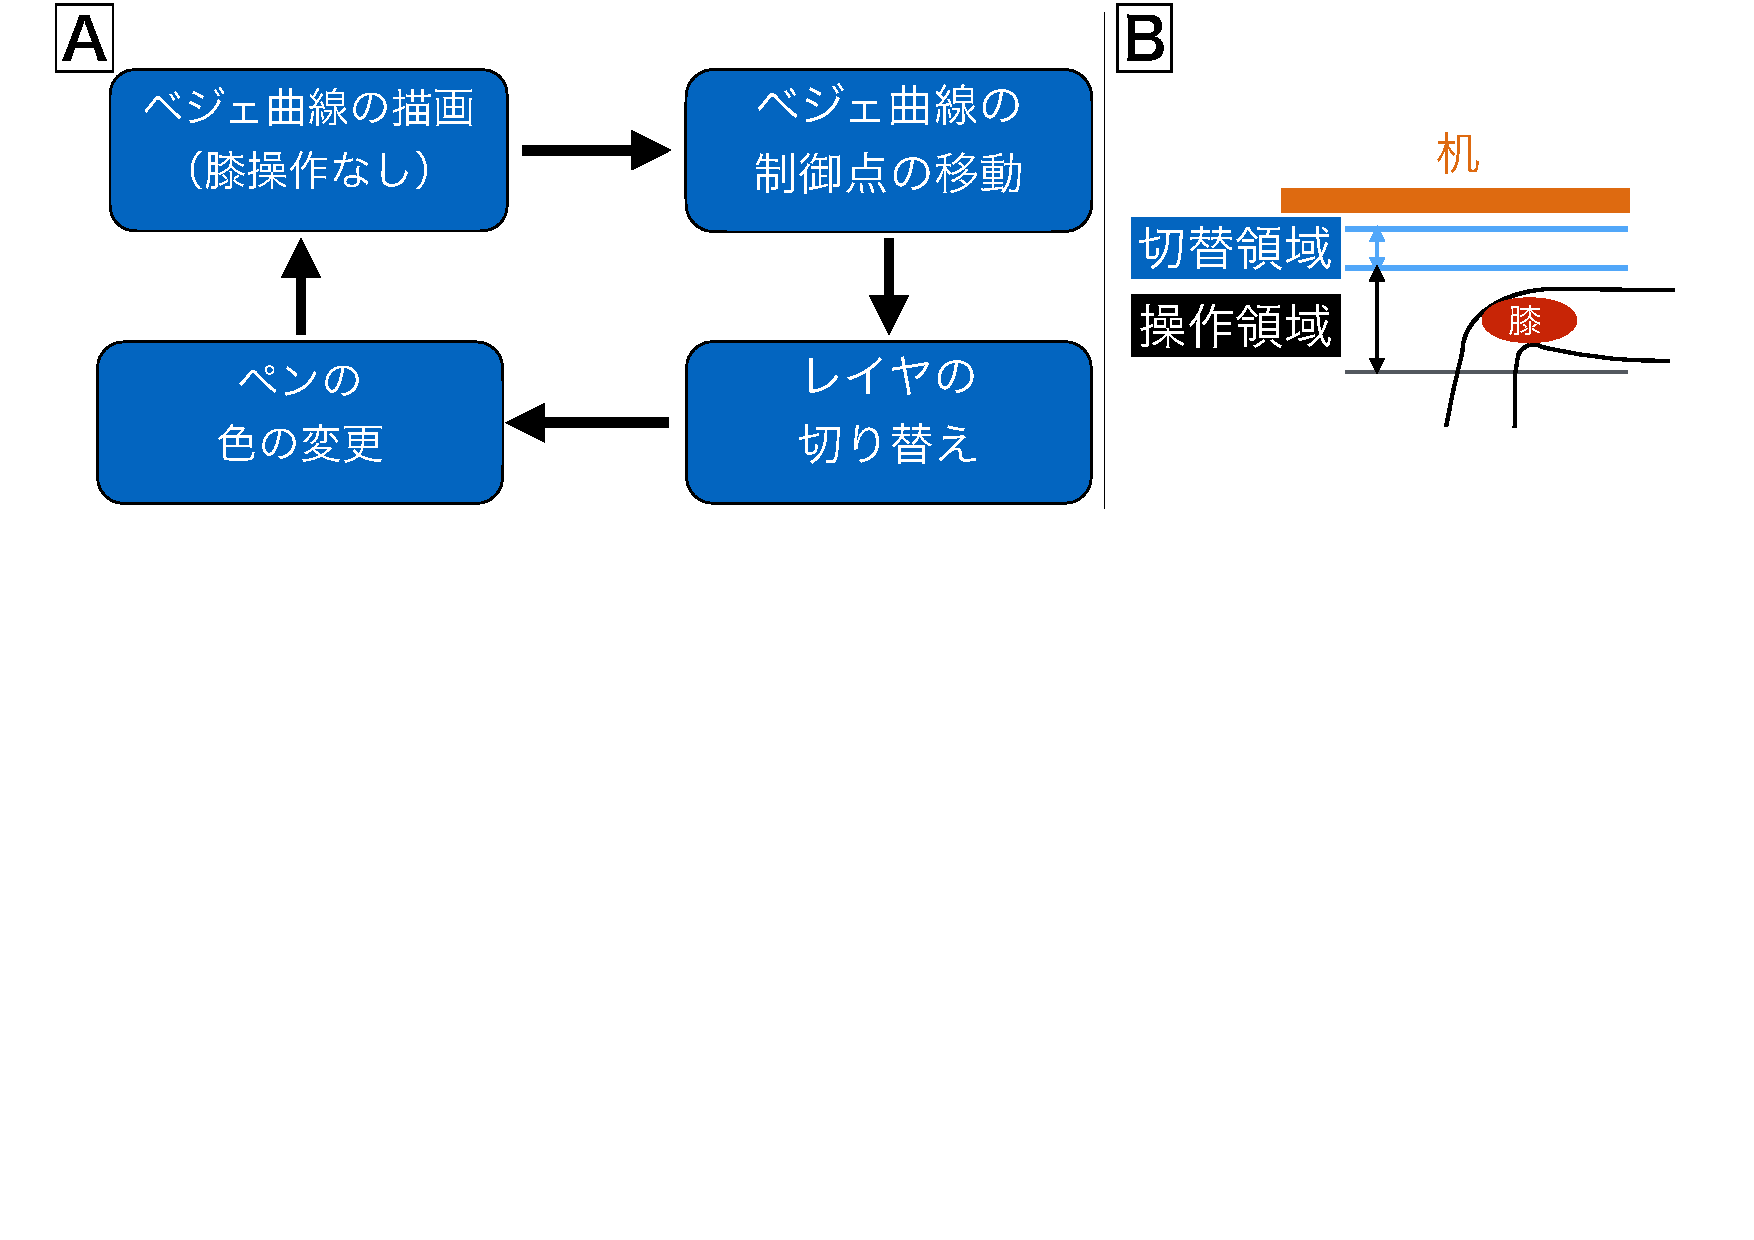
\includegraphics[width = 1.0\hsize]{./figures/statements.pdf}
%	\end{center}
%	\caption{膝によって切り替わる各操作の状態遷移図.}
%	\label{img:statements}
%\end{figure}
\img{H}{1.0}{statements.pdf}{膝によって切り替わる各操作の状態遷移図.}{statements}
\img{h}{1.0}{switch_operation_area.pdf}{ユーザの膝と操作領域および切り替え領域の関係}{switch_operation_area}

\subsection{キャリブレーション}
本プログラムはユーザが簡単に膝操作を使えるように,起動時に膝位置のキャリブレーションを行う.
キャリブレーションに際して,ユーザは膝が直角になるように座り,距離センサアレイの範囲内に膝を合わせる.プログラムを起動すると自動でキャリブレーションが行われる.
プログラムでは,ユーザの左右方向の膝の位置と上下方向の膝の位置を20回ずつ取得し,それぞれの平均値を保存する.
この時ユーザは動かないように注意する.キャリブレーションが終了すると自動で開始画面が表示される.
キャリブレーションを行うことで,前述の操作領域が決定する.
操作領域はキャリブレーション時のユーザの膝の位置を中心として,左右方向に約1.5 \si{cm},上方向に約2.0 \si{cm},下方向に約1.0 \si{cm}の範囲となる.

\section{予備実験}
ユーザが膝操作によって区別可能な,操作領域の分割数を調査するための予備実験を行った.この実験は3名(男性1名,女性2名)の参加者に対し行った.

\subsection{実験条件・タスク}

\refImg{preex_window}は本実験にて使用したプログラムの画面一例である.参加者にはいくつかの長方形(セクション)が表示されている.参加者は膝を上下または左右に動かすことで,緑色のセクション(ポインタ)の位置を移動することができる.ポインタを移動させて青色のセクション(ターゲット)に重ね,Enterキーを押す(=1選択操作).実験は以下の条件について行った.
\begin{itemize}
	\item{膝の操作方向:}左右,上下
	\item{セクションの数:}5,10,15,20
	\item{現在のポインタの位置:}見える(可視条件),見えない(不可視条件)
\end{itemize}
1条件につき選択操作は20回ずつ行われる.5分割の時は4回、10分割の時は2回同じセクションがターゲットとなり,15分割の時はランダムに5つのセクションが2回ターゲットとなる。また,セクション数によって1つのセクションの幅(左右方向の時)と高さ(上下方向の時)は\refTb{section_width_height}のように変化する.
\img{h}{1.0}{preex_window.pdf}{予備実験にて使用したプログラムの画面一例(膝の操作方向:左右,セクション数:10,可視条件).}{preex_window}
\begin{table}[h]
	\caption{1つのセクションの幅または高さの対応}
	\label{tb:section_width_height}
	\begin{center}
		\begin{tabular}{c|c|c}
			セクション数 & \begin{tabular}[c]{@{}c@{}}左右方向の時の幅\\ (ピクセル)\end{tabular} & \begin{tabular}[c]{@{}c@{}}上下方向の時の高さ\\ (ピクセル)\end{tabular} \\ \hline
			5      & 216                                                       & 124                                                        \\ 
			10     & 108                                                       & 62                                                         \\
			15     & 72                                                        & 41.3                                                       \\ 
			20     & 54                                                        & 31                                                        
		\end{tabular}
	\end{center}
\end{table}
\subsection{収集データ}
データ数の合計は,
$2$(操作方向) $\times 4$(分割数) $\times 2$(可視/不可視条件) $\times 20$(操作回数) $\times 3$ (参加者) $= 960$
であった.1データにつき,選択操作の正誤,操作に要した時間を収集した.実験全体では参加者1人あたり30分程度で終了した.

%\subsection{実験手順}
%まず,参加者は一方の膝を距離センサアレイの中心位置に合わせてから椅子に座る.次に実験実施者がプログラムを起動する.参加者の膝の位置を認識していることを確認したら,参加者が実験開始キーを押して計測を開始する.
\subsection{実験結果}
\refImg{preex_results}は予備実験における平均正解率,平均操作時間のグラフである.縦軸は,平均正解率のグラフでは正解率($\%$),平均操作時間のグラフでは操作時間(秒)を表す.横軸は分割数を表す.平均操作時間のグラフのエラーバーは標準偏差を表す.ただし,平均操作時間のグラフでは10秒以上かかっていたデータを外れ値として除外している.
可視条件では,5または10分割においては,平均90\%以上の正解率であった.15または20分割でも80\%以上の正解率であった.したがって,20分割程度であれば問題なく操作可能であることがわかる.また平均操作時間は5または10分割では2秒以内,15または20分割でも3秒以内であった.後述する膝操作のGUIへの適用実験では,特に操作時間,正解数共に良好な10分割程度で実験を行うこととした.
\par
また不可視条件では,平均正解数は8条件中7条件で50\%に満たなかった.一方,平均操作時間は操作方向ごとに同程度で,かつ可視条件での5または10分割と同程度であった.原因を調査するために,各ターゲットの中央の座標を基準とした時の膝の位置の平均誤差を調査した(\refImg{preex_diff}).
\img{b}{1.0}{preex_results_3.pdf}{予備実験における平均正解率,平均操作時間の結果.}{preex_results}
グラフの縦軸は,選択操作をした時のターゲットとのずれをピクセル(上段)とセクション数(下段)を表している.横軸は分割数を表す.エラーバーは標準偏差を表す.
不可視条件の場合のピクセルでの誤差は,平均して左右方向で100ピクセル以上,上下方向で150ピクセル以上の誤差があった.しかし分割数ごとに大きく差はなかった.
またセクション数では,各分割数において左右方向では最小0.3セクション(セクション数5),最大4.4セクション(セクション数20),上下方向では最小0.5セクション(セクション数5),最大9.9セクション(セクション数20)の誤差があった.\par
さらに不可視条件のとき,参加者がどのセクションを選択していたかを調べるため,各セクションの誤選択を含めた合計選択回数を調査した(\refImg{preex_selection_times}).
結果,どの分割数においても両端のセクションが選択されている傾向があることがわかった.
%\vspace{-0.4cm}
\img{h}{1.0}{preex_diff_3.pdf}{不可視条件における選択時の膝位置の平均誤差}{preex_diff}
\img{H}{1.0}{preex_selection_times.pdf}{不可視条件における各セクションの選択回数合計}{preex_selection_times}
\par

\subsection{考察}
結果から,参加者は大まかに全てのセクションを半分に分けて,ターゲットが左(上)にある時と右(下)にある時で膝を左(上)方向,右(下)方向に動かしていたと推測される.加えて操作領域が十分大きくなかったことで,両端のセクションの選択回数が多くなり,ピクセル数の誤差も分割数にかかわらず一定であったと考えられる.
%また1条件の選択回数はどの分割数でも20回ずつなので,各セクションがターゲットになる回数は,5分割の場合4回ずつ,10分割の場合2回ずつ,15分割の時に1または2回ずつ,20分割の時に1回ずつである.したがって参加者の膝の左右(上下)の方向のみがあっていた場合,正解率はそれぞれ40\%,20\%,10\%,10\%程度になると考えられ,これは\refImg{preex_results}で示された結果にほぼ一致している.\par
今後操作領域が大きくなるようにキャリブレーション方法を見直すと共に,5分割未満の条件を追加して再実験を行い,不可視条件における膝の操作性を詳しく調査する.
\section{膝操作のGUIへの適用実験}
実装したベジェ曲線描画プログラムを通して,膝操作をGUIへ適用した時の使用感を調査する目的で実験を行った.この実験によって膝操作が適合する操作,およびアプリケーション実装上での指針を明らかにする.
\subsection{参加者}
参加者は合計6名(男性5名,女性1名)である.まず2名に対し実験を行ったところ,レイヤ切替モードとペンの色変更モードにおいて,操作を切り替える瞬間にレイヤやペンの色が変化してしまうという問題があることがわかった.対策として,Shiftキーを押している間は2つのモードにおいてレイヤや色の変更を停止し,モードの切り替えのみを行うことができるように実装を変更した.

\subsection{実験タスク}
実験に際して,アニメーション描画タスクを設計した.これは,10フレームの「夕陽が沈む」アニメーションを作成してもらう.\refImg{animation_example}はアニメーションの一例であり,各フレームの丸が太陽,波線が波を表している.1フレームごとに太陽の位置が徐々に波に沈むように変化させ,同時に線の色も黄色から赤に変化させる.1レイヤに対し1フレームを描く.また,参加者にはあらかじめ著者が用意した1フレーム目の見本をトレースまたは書き写し,10フレーム目には波だけ(\refImg{animation_example}右下)を描くように指示した.加えて参加者には絵の優劣は実験とは関係ないことを注意した.
\img{h}{1.0}{animation_example}{アニメーション描画タスクで描かれるアニメーション一例.}{animation_example}
\subsection{実験手順}
まず参加者は椅子に座り,左右どちらの膝を使うかを選択する.実験者は参加者の着座位置と膝の左右に応じて,参加者の膝が距離センサアレイの真ん中になるように位置を調整する.次に,実験者がプログラムを実際に操作しながら,参加者にプログラムの操作と,アニメーション描画タスクについて説明を行う.その後5分間の練習タスクを行う.練習タスクでは,アニメーション描画タスクを2,3フレーム程度行い,プログラムの操作や膝での操作に慣れてもらう.その後本番タスクを行う.
本番タスクは次の2通りにおいてアニメーションの作成を行う.
\begin{enumerate}
	\item マウス操作のみで行う
	\item マウス操作と膝操作を組み合わせて行う
\end{enumerate}
参加者間で1,2のタスクの順番はランダムとした.1回のタスクの制限時間は15分程度としたが,参加者が自分の作品に満足であれば,15分より早く終了することを許可した.本番タスク終了後に自由記述によるアンケートを実施した.またタスク間では5分間の休憩をとった.
\subsection{収集データ}
本番タスク中のマウスカーソル座標,膝の座標,膝の操作モードを,いずれかが変化した時のイベントを用いてタイムスタンプ付きで記録した.これらを組み合わせたデータ1つを1レコードと呼ぶ.参加者1人あたり約20000〜50000レコードを収集した.また,参加者の後方からビデオ撮影し,膝操作の様子を記録した.さらに自由記述によるアンケートを行い,どのような操作が好ましいかなどの意見を募った.

\subsection{実験結果}
%各モードで参加者の意見,実験ビデオ,座標の記録から総合して,「ペン色変更モード」,「レイヤ切替モード」,「制御点移動モード」の順でよく使われ,参加者からの印象も良かった.
%まず「ペン色変更モード」は,実験中に使用された時間の長さが最も長く,全参加者の平均34.3\%の時間で使用されていた.また,「ペン色変更モード」にしたまま操作モードを切り替えずに行った参加者も1名おり,アンケートでは「最も使えて嬉しい機能だった」と回答した.
%次に「レイヤ切替モード」は,全参加者の平均6.8\%の時間で使用された.プログラム改良後に参加した1名は,操作時間の19.2\%の間使用し,アンケートでも「レイヤの変更を膝で行うことは便利だった」と回答した.一方で,マウスでのみ切り替えを行う参加者も複数存在していた.またある参加者は,アンケートで「レイヤを一覧表示するテーブルのスクロールのみを膝で行いたい」と回答した.
%最後に制御点移動モードはほとんど使用されておらず,全参加者で平均1.2\%の時間でしか使用されなかった.参加者からも,アンケートにて「点を動かすのにはどうだろう」と疑問符がつく意見があった.\par
%また,モードを切り替え操作において意図しない切り替えが発生している,切り替え操作において参加者によっては足を大きく浮かす必要があったこともわかった.1名の参加者は「モード切り替えが1つずつしか進まないのが難しかった」と述べていた.
\begin{table}[h]
	\caption{各操作モードの実験時間に占める割合.}
	\label{tb:mode_time}
	\begin{center}
		\begin{tabular}{c|c}
			操作モード    & 実験時間に占める割合 \\ \hline
			ベジェ曲線の制御点の移動 & 1.4\%      \\ 
			レイヤの切り替え & 8.4\%      \\
			ペンの色の変更 & 34.2\%     \\ 
		\end{tabular}
	\end{center}

\end{table}
\refTb{mode_time}は3つの操作モードが使用された時間の,実験時間に占める割合を表している.3つの操作モードの中では,「ペンの色の変更」が最も使われた時間が長かった.対して,「ベジェ曲線の制御点の移動」はほとんど使われていなかった.また2つのタスクにおける平均の実験時間は,マウス操作のみで行った場合は12分02秒,マウス操作と膝操作を組み合わせて行った場合は14分06秒であった.\par
アンケートでは,レイヤ切り替え操作については「レイヤの変更を膝で行うのは便利だった」と好意的な意見があった一方,「選択ではなく,表示のスクロールだけを変更できた方が良いと感じた」という,膝をマウスの補助としたいという意見も得られた.ペンの色の選択についても,「レイヤの変更を膝で行うのは便利だった」と好意的な意見の一方で,「色の細かいところを膝で選ぶのが難しかった」,「色の調整はマウスの方がしやすいと思った」と,膝で操作することが難しいと感じる意見も得られた.また,「ベジェ曲線の制御点の移動」では「点を動かすのにはどうなんだろう」と疑問符を浮かべる意見があった.さらに膝による操作に切り替えに関して,「モード切り替えが1つずつしか進まないのが難しかった」といった意見も得られた.

\subsection{考察}
実験結果より,「レイヤの切り替え」と「ペンの色の変更」については好意的な意見も得られたことから,「リスト選択」と「スライダ操作」は膝操作に適合する可能性があると考えられる.しかし膝操作が難しいという意見や,選択ではない操作に使いたいという意見もあることから,膝操作をマウスの補助あるいはマウスを膝操作の補助に用いることが適する可能性もある.
これに対して,「ベジェ曲線の制御点の移動」はあまり使われず印象も悪かった.これは,今回行ったアニメーション描画タスクでは単純な絵であったために必要がないと判断されたこと,絵のクオリティを不問としていたため精密に調整する必要がなかったことが原因として挙げられる.
また,実験時間がマウス操作のみで行った場合より,マウス操作と膝操作を組み合わせた場合の方が平均2分程度長くなった.原因の1つとしては練習タスクの長さが不十分であり,参加者が十分に膝操作やプログラムに慣れることができていなかったことが考えられる.また,レコードやビデオを確認すると膝での操作の切り替えの誤発火があり,目的の操作に修正するのに時間を取られていたことから,操作の切り替えがうまくいかなかったことも原因であると考える.
\section{まとめと今後の課題}
本稿ではこれまで未検証であった,膝操作の一般的なGUI操作への適用可能性を探った.カーソル操作,テーブル操作,スライダ操作を対象とし,GUIアプリケーションの一例としてベジェ曲線描画プログラムを実装した.それぞれの操作は,「ベジェ曲線の制御点の移動」,「レイヤの切り替え」,「ペンの色の変更」として対応させた.また実装したプログラムを用いてアニメーション描画タスクを行い,膝操作をGUI操作に適用した時の使用感,指針を調査した.実験の結果,スライダ操作が膝操作に適合する可能性が高いことがわかった.一方で,カーソル操作はマウスで行った方が良いこともわかった.これらの結果と,モード切り替えにおける知見を総合して,膝操作によるアプリケーション実装の指針を示した.\par
今後の課題として,実験結果を踏まえたより詳細な調査を行う.まず「リスト選択」と「スライダ操作」について,膝操作とマウス操作のどちらを主な入力とするのがふさわしいかを調査する必要がある.さらに,「見本を忠実に再現した絵を描く」といった精密な操作を必要とするタスクによって,「ベジェ曲線の制御点の移動」の適合性をさらに調査する.また操作切り替えの誤発火について詳しく調査し,膝での操作切り替えを見直すことによって,マウスのみの操作と同等の操作時間を目指す.加えて,マウスなど既存のデバイスと膝操作とを併用した,新たな操作やインタラクションの探究を行う.
\par
%% bib
\bibliographystyle{ipsjunsrt}
%\bibliographystyle{ipsjsort}
%\bibliographystyle{junsrt}
%\bibliography{bibsample}
\bibliography{ref.bib}



\begin{biography}

\end{biography}



\end{document}
